\documentclass[]{article}

% Imported Packages
%------------------------------------------------------------------------------
\usepackage{amssymb}
\usepackage{amstext}
\usepackage{amsthm}
\usepackage{amsmath}
\usepackage{enumerate}
\usepackage{fancyhdr}
\usepackage[margin=1in]{geometry}
\usepackage{graphicx}
\usepackage{extarrows}
\usepackage{setspace}
\usepackage{placeins}
\usepackage{float}
%------------------------------------------------------------------------------

% Header and Footer
%------------------------------------------------------------------------------
\pagestyle{plain}  
\renewcommand\headrulewidth{0.4pt}                                      
\renewcommand\footrulewidth{0.4pt}               
%------------------------------------------------------------------------------

% Title Details
%------------------------------------------------------------------------------
\title{Deliverable \#2 Template}
\author{SE 3A04: Software Design II -- Large System Design}
\date{}                               
%------------------------------------------------------------------------------

% Document
%------------------------------------------------------------------------------
\begin{document}

\maketitle	

\section{Introduction}
\label{sec:introduction}
% Begin Section

This document will go in depth into the design of Merlin, a song lookup application, using various different analysis methods such as a Use Case Diagram, Analysis Class Diagram, Architectural Design Analysis, as well as Class Responsibility Collaboration (CRC) Cards.

\subsection{Purpose}
\label{sub:purpose}
% Begin SubSection
	The purpose of this documentation is to state, describe and analyze the architecture of the Merlin song identification app. This will be done through a set of predetermined and proven analysis methods and is intended to be read by the implementation team and client. 
% End SubSection

\subsection{System Description}
\label{sub:system_description}
% Begin SubSection
	The application, Merlin, contains a back end system that will be discussed in this report. The system is constructed using multiple expert classes and each class will render a different set of code. A user may input the information about a song using the Tempo, Lyric or using the Artists name. The app will then use these experts to find the song that the user is trying to search for from a database of all songs. The user will have their previous search information stored on the device. This application will run on any android application, and will be available for download through the android app store.
% End SubSection

\subsection{Overview}
\label{sub:overview}
% Begin SubSection
This document has 5 sections including this one. Every section analyzes the architecture of the Merlin application’s system in a different way using either diagrams or words. Following is a breakdown of what each section analyzes: 
\begin{enumerate}[1)]
	\item Use Case Analysis and Diagram: This section will demonstrate all possible ways of the app’s interaction with the user. 
	\item Analysis Class Diagram: This diagram will outline the three different types of classes (boundary, controller or entity) and specify which class falls under which category. This section will also show the different connections between the classes.
	\item Architectural Design Class: This section will overview and justify the reason for designing the application in the chosen way. 
	\item Class Responsibility Collaboration Cards: These cards will show the different classes that make up the song identification app, and their key responsibilities. It will also state which classes each other interact with. 
\end{enumerate}
% End SubSection

% End Section

\section{Use Case Diagram}
\label{sec:use_case_diagram}
% Begin Section
\begin{figure}[!ht]
	\centering
	\includegraphics[scale=1]{UseCaseDiagram.png}
	\caption{Use Case Diagram}
\end{figure}
\begin{description}
	\item[View Previous Searches] The user must be able to review their previous searches. All searches should be saved so that they may be displayed in this list. The data saved should consist of the inputs entered to return the result.
	\item[Get More Song Info] Each song result is linked to more detailed information about the artist and song. The user should have access to this more detailed information on request. This use case cannot be executed unless a song is searched for first.
	\item[Search for Song] The user can search for a song based on the inputs given.
	\item[Input] This use case is a generic use case that is extended by more specific input fields. These fields include Tempo Input, Lyric Input and Artist Input.
	\item[Tempo Input] To input a tempo the user must tap on the screen at the desired tempo. This tempo is converted to a measurement in BPM for searching.
	\item[Lyric Input] To input lyrics users will have the option to type some lyrics into the search field or speak into the device's microphone and translate their voice to text via the speech-to-text functionality. These lyrics are a sequence of words that can be found in the desired song.
	\item[Artist Input] The artist input is the name of the artist that preforms the desired song. To input the artist the user may type the name into the search field or speak into the device's microphone and translate their voice to text via the speech-to-text functionality.
	\item[Consult Experts] Experts will be consulted to attempt to identify the desired song. They will work together to combine their opinions to decide on a song.
	\item[Add/Remove Expert] The administrator may wish to take an expert out of the system or introduce an new expert. In order to do so they must contact the developer who will directly preform the switch. 
\end{description}
\FloatBarrier % Stop the figure from leaving the section
% End Section

\section{Analysis Class Diagram}
\label{sec:analysis_class_diagram}
% Begin Section
\subsection{Noun Extraction}
\begin{description}
	\item[user] No (outside of system)
	\item[previous searches] Yes (boundary class) PreviousSearchPage
	\item[searches] refers to search process, leads to the creation of controller class SearchController
	\item[success] Yes (boundary class) SearchSuccessPage or SearchResults
	\item[error] Yes (boundary class) SearchErrorPage
	\item[song info] Yes (entity class) SongInformation
	\item[input] refers to input process, leads to the creation of controller class InputController
	\item[tempo input] Yes (boundary class)
	\item[lyric input] Yes (boundary class)
	\item[artist input] Yes (boundary class)
	\item[song database] Yes (boundary class), Wrapper
\end{description}

\begin{figure}[!ht]
	\centering
	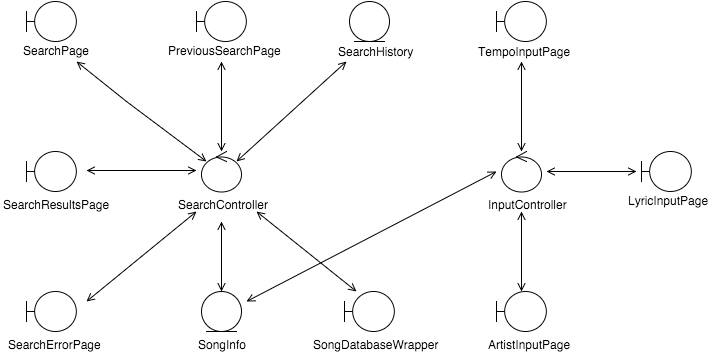
\includegraphics[scale=0.7]{Analysis_Class_Diagram.png}
	\caption{Analysis Case Diagram}
\end{figure}
\FloatBarrier
% End Section


\section{Architectural Design}
\label{sec:architectural_design}
% Begin Section

\subsection{System Architecture}
\label{sub:system_architecture}
% Begin SubSection
\begin{enumerate}[a)]
	\item A blackboard architectural design will be used.
	\item The system will primarily use the information obtained by 3 experts to determine a final result. The nature of this structure lends itself to the chosen type architecture.
\begin{figure}[H]
	\centering
	\includegraphics[width=\textwidth,keepaspectratio]{architecture.png}
	\caption{System Architecture Diagram}
\end{figure}
\end{enumerate}
% End SubSection

\subsection{Subsystems}
\label{sub:subsystems}
% Begin SubSection
\begin{enumerate}[a)]
	\item \textbf{Artist Expert:} The expert charged with identifying songs associated with a given artist.
	\item \textbf{Lyric Expert:} The expert charged with identifying songs associated with a given lyric.
	\item \textbf{Tempo Expert:} The expert charged with identifying songs associated with a given tempo.
	\item \textbf{Blackboard:} The subsystem charged with combining data from all other subsystems and producing a final result for the user interface.
	\item \textbf{User Interface:} The subsystem charged with handling interactions with the user, including input and output.
\end{enumerate}
% End SubSection

% End Section
	
\section{Class Responsibility Collaboration (CRC) Cards}
\label{sec:class_responsibility_collaboration_crc_cards}
% Begin Section
	\begin{table}[!htb]
		\centering
		\begin{tabular}{| p{8cm} | c |} \hline
			\multicolumn{2}{|l|}{\textbf{Class Name: InputController}} \\ \hline
			\textbf{Responsibility:} & \textbf{Collaborators:} \\ \hline
			Handle inputted tempo data & TempoInputPage \\ \hline
			Handle inputted song lyrics & LyricInputPage \\ \hline
			Handle inputted artist name & ArtistInputPage \\ \hline
			Send data to be stored and used for searches & SongInfo \\ \hline
		\end{tabular}
	\end{table}
	
	\begin{table}[!htb]
		\centering
		\begin{tabular}{| p{8cm} | c |} \hline
			\multicolumn{2}{|l|}{\textbf{Class Name: TempoInputPage}} \\ \hline
			\textbf{Responsibility:} & \textbf{Collaborators:} \\ \hline
			Convert user input into beats per minute &   \\ \hline
			Relay information to the InputController & InputController \\ \hline
		\end{tabular}
	\end{table}
	
	\begin{table}[!htb]
		\centering
		\begin{tabular}{| p{8cm} | c |} \hline
			\multicolumn{2}{|l|}{\textbf{Class Name: LyricInputPage}} \\ \hline
			\textbf{Responsibility:} & \textbf{Collaborators:} \\ \hline
			Temporarily store user string inputs &   \\ \hline
			Relay data to the InputController & InputController \\ \hline
		\end{tabular}
	\end{table}
	
	\begin{table}[!htb]
		\centering
		\begin{tabular}{| p{8cm} | c |} \hline
			\multicolumn{2}{|l|}{\textbf{Class Name: ArtistInputPage}} \\ \hline
			\textbf{Responsibility:} & \textbf{Collaborators:} \\ \hline
			Temporarily store user string inputs &   \\ \hline
			Relay data to the InputController & InputController \\ \hline
		\end{tabular}
	\end{table}
	
	\begin{table}[!htb]
		\centering
		\begin{tabular}{| p{8cm} | c |} \hline
			\multicolumn{2}{|l|}{\textbf{Class Name: SearchHistory}} \\ \hline
			\textbf{Responsibility:} & \textbf{Collaborators:} \\ \hline
			Process search history requests & SearchController \\ \hline
			Store previous search results &   \\ \hline
			Order searches by time of search &   \\ \hline
		\end{tabular}
	\end{table}
	
	\begin{table}[!htb]
		\centering
		\begin{tabular}{| p{8cm} | c |} \hline
			\multicolumn{2}{|l|}{\textbf{Class Name: SongDatabaseWrapper}} \\ \hline
			\textbf{Responsibility:} & \textbf{Collaborators:} \\ \hline
			Produce results based of given search queries & SearchController \\ \hline
			Store data on song lyrics, artists, and tempos &   \\ \hline
			Order song data based of date of release &   \\ \hline
		\end{tabular}
	\end{table}
	
	\begin{table}[!htb]
		\centering
		\begin{tabular}{| p{7cm} | c |} \hline
			\multicolumn{2}{|l|}{\textbf{Class Name: SearchController}} \\ \hline
			\textbf{Responsibility:} & \textbf{Collaborators:} \\ \hline
			Perform search use case & SearchPage \\ \hline
			Inform SongInfo of search results & PreviousSearchPage \\ \hline
			Inform SearchHistory of search results & SongInfo \\ \hline
			& SearchHistory \\ \hline
			& SearchDatabaseWrapper \\ \hline
			& SearchErrorPage \\ \hline
			& SearchResultsPage \\ \hline
		\end{tabular}
	\end{table}
	
	\begin{table}[!htb]
		\centering
		\begin{tabular}{| p{8cm} | c |} \hline
			\multicolumn{2}{|l|}{\textbf{Class Name: SearchErrorPage}} \\ \hline
			\textbf{Responsibility:} & \textbf{Collaborators:} \\ \hline
			Read information on error page & SearchController \\ \hline
			Inform SearchController of information on error page &   \\ \hline
		\end{tabular}
	\end{table}
	
	\begin{table}[!htb]
		\centering
		\begin{tabular}{| p{8cm} | c |} \hline
			\multicolumn{2}{|l|}{\textbf{Class Name: SearchResultsPage}} \\ \hline
			\textbf{Responsibility:} & \textbf{Collaborators:} \\ \hline
			Read information on results page & SearchController \\ \hline
			Inform SearchController of information on results page &   \\ \hline
		\end{tabular}
	\end{table}
	
	\begin{table}[!htb]
		\centering
		\begin{tabular}{| p{8cm} | c |} \hline
			\multicolumn{2}{|l|}{\textbf{Class Name: SearchPage}} \\ \hline
			\textbf{Responsibility:} & \textbf{Collaborators:} \\ \hline
			Read information on search page & SearchController \\ \hline
			Inform SearchController of information on the page &   \\ \hline
		\end{tabular}
	\end{table}
	
	\begin{table}[!htb]
		\centering
		\begin{tabular}{| p{8cm} | c |} \hline
			\multicolumn{2}{|l|}{\textbf{Class Name: PreviousSearchPage}} \\ \hline
			\textbf{Responsibility:} & \textbf{Collaborators:} \\ \hline
			Read information on previous search page & SearchController \\ \hline
			Inform SearchController of information on the previous search page &   \\ \hline
		\end{tabular}
	\end{table}
	
	\begin{table}[!htb]
		\centering
		\begin{tabular}{| p{8cm} | c |} \hline
			\multicolumn{2}{|l|}{\textbf{Class Name: SongInfo}} \\ \hline
			\textbf{Responsibility:} & \textbf{Collaborators:} \\ \hline
			Inform SearchController of users search query and wait for results & SearchController \\ \hline
			Display to user, results of the song search & InputController \\ \hline
			Inform InputController when a search is completed &   \\ \hline
		\end{tabular}
	\end{table}

% End Section

\appendix
\section{Division of Labour}
\label{sec:division_of_labour}
% Begin Section
Include a Division of Labour sheet which indicates the contributions of each team member. This sheet must be signed by all team members.
% End Section

\end{document}
%------------------------------------------------------------------------------